\chapter{Introducción}\label{cap.introduccion}
%\pagenumbering{arabic} % para empezar la numeración con números
\section{Contexto}
Desde el surgimiento de la primera generación de comunicaciones móviles \ac{1g}, la impronta de estas comunicaciones se ve reflejada hasta en el más mínimo aspecto de la vida cotidiana y de la industria. Lejos ha quedado ya la tradicional y exclusiva utilidad de realizar llamadas de voz que tenían los terminales móviles en un principio.

\begin{figure}[hb]
	\centering
    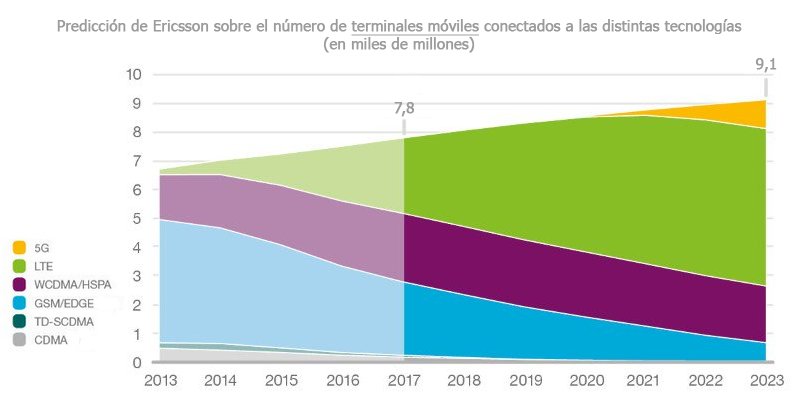
\includegraphics[width=1\linewidth]{imagenes/5gforecast.PNG}
	\caption{Suscripciones móviles por tecnología (en miles de millones) \cite{5gForecastEricsson}}
	\label{fig:5gforecast}
\end{figure}

Con la aparición de las siguientes generaciones, el uso de datos móviles se ha convertido en la finalidad principal de estos dispositivos. Según \cite{informeInicial}, ``El móvil es el dispositivo más utilizado en España para acceder a internet, usado ya por el 94,6 \% de los españoles", asimismo, según la previsión de Cisco \cite{informeInicialCisco}, para el año 2021 existirá un total de 11,6 miles de millones de dispositivos, tanto terminales móviles como otros tipos de dispositivos, conectados a la red móvil en todo el mundo. Esto supondría un tráfico mensual de alrededor de 50 Exabytes a través de la infraestructura de comunicaciones móviles -tres veces más tráfico que en la actualidad-.

\subsection{El futuro de las redes inalámbricas. 5G, \textit{hetnets} y Horizonte 2020}

Con el propósito de hacer frente a las características que las infraestructuras de red han de reunir en el futuro, resultan cruciales las labores de investigación y desarrollo para el establecimiento de nuevos estándares que permitan la coexistencia de dispositivos de distinta naturaleza, ya que las actuales tendencias hacen que empiece a surgir la distinción entre Internet de terminales móviles e Internet de las Cosas, \ac{iot}, siendo de esperar que el número de dispositivos conectados crezca considerablemente año tras año.


Actualmente, es la comunicación de quinta generación, \ac{5g} el estándar que se encuentra en pleno desarrollo y que será el sucesor de la cuarta generación, \ac{4g}. Este estándar pretende ofrecer servicios con una muy alta capacidad, conectividad masiva, muy baja latencia, muy alta seguridad, consumo de energía muy bajo y una calidad de servicio, \ac{qos} extremadamente alta \cite{comparative5G}.

\begin{table}[h]
\centering
\caption{Objetivos de 5G \cite{cognitive5G}.}
\label{tab:5gfeatures}
\resizebox{\textwidth}{!}{%
\begin{tabular}{@{} >{\centering\arraybackslash}m{2.5cm} >{\centering\arraybackslash}m{3.5cm} m{7cm} @{}}
\toprule
\multicolumn{2}{c}{\textbf{Escenario de Aplicación}}    & \multicolumn{1}{c}{\textbf{Requisitos y Desafíos}}                                                                                                         \\ \midrule
\multirow{2}{*}[-17pt]{Internet móvil} & Cobertura extensa & Ofrecer un servicio de alta velocidad, en cualquier momento, en cualquier sitio y en escenarios difíciles como áreas remotas.                              \\ \cmidrule(l){2-3} 
                                & Capacidad masiva      & Ofrecer servicio a usuarios con ratios de transmisión extremadamente altos, y hallar las características que las redes de alto flujo de datos necesitarán. \\ \midrule
\multirow{2}{*}[-30pt]{IoT}            & Conectividad masiva   & Ofrecer capacidad para más de un millón de conexiones simultáneas, y asegurar a los terminales un consumo extremadamente bajo de energía.                  \\ \cmidrule(l){2-3} 
                                & Baja Latencia         & Ofrecer a los usuarios un retardo de menos de 1 milisegundo punto a punto, y cerca de un 100\% de fiabilidad.                                                       \\ \bottomrule
\end{tabular}%
}
\end{table}

En concreto, 5G propone un enfoque disruptivo de las comunicaciones. Debido a la gran cantidad de terminales que estarán conectados simultáneamente y su constante expansión, es primordial ofrecer servicio a todos ellos, tanto en entornos con una densidad de usuarios extremadamente alta como en entornos rurales en los que existe una mayor dispersión de usuarios. Para ello, los operadores pretenden ampliar el rendimiento de sus servicios a través de sistemas multiantena utilizando tecnología \ac{mimo} y mediante técnicas de modulación y multiplexación más eficientes, al mismo tiempo que se aumenta el ancho de banda y se utilizan frecuencias mucho más altas.


\begin{figure}[ht]
	\centering
    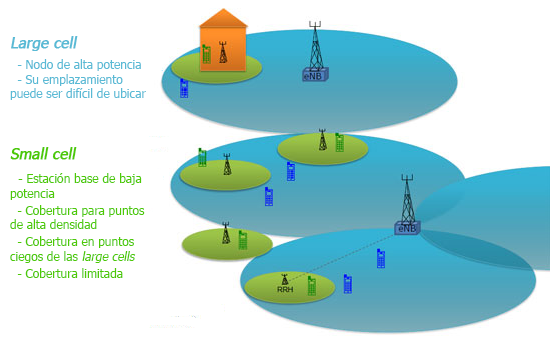
\includegraphics[width=1\linewidth]{imagenes/hetnet_enviroment.png}
	\caption{Entorno típico de \acs{hetnet} \cite{hetnetexplained}}
	\label{fig:hetnet}
\end{figure}

Sin embargo, este conjunto de técnicas y adaptaciones no son suficientes para soportar el uso extremadamente intenso que recibirán las infraestructuras. Por ello, un concepto muy importante en 5G es el de \textit{\acl{hetnet}} (\acs{hetnet}), o lo que es lo mismo, redes heterogéneas en las que conviven nodos o puntos de acceso de diferentes características. En las redes heterogéneas las celdas cuentan con un diferente tamaño según su tipo. De este modo, se distingue entre \textit{macro-, micro-, pico-} y \textit{femto-celdas}. La única diferencia entre ellas a priori es el área de cobertura, la cual es definida mediante la variación de la frecuencia, de la potencia de transmisión y de la altura a la que se encuentra la estación base de la celda en cuestión.


\begin{table}[ht]
\centering
\caption{Características de las clases de celdas.}
\label{tab:celdas}
\begin{tabular}{m{3cm} m{9cm}}
\hline
\multicolumn{1}{c}{\textbf{Tipo de celda}} & \multicolumn{1}{c}{\textbf{Características}}                                                                                                             \\ \hline
Femto-celda                                & Son autónomas y tienen capacidad para apenas unos pocos usuarios. El área que puede cubrir es muy reducida.                                              \\ \hline
Pico-celda                                 & Pueden soportar hasta 100 usuarios simultáneos en áreas de menos de 200 metros. Normalmente se usan en interiores.                                       \\ \hline
Micro-celda                                & De uso urbano, estas celdas pueden cubrir áreas de hasta 1,5 km. En la actualidad, se utilizan para proporcionar cobertura adicional en eventos masivos. \\ \hline
Macro-celda                                & Se puede comparar con las celdas tradicionales. Ofrecen una cobertura máxima de unos 30 km.                                                              \\ \hline
\end{tabular}
\end{table}


A modo de simplificación, se suele utilizar el término \textit{small cell} para hacer referencia a cualquier celda que no sea del tipo \textit{macro-celda}. Se puede comprender un escenario típico de red heterogénea a través de la ilustración de la figura \ref{fig:hetnet}. Como explica dicha figura, en el paradigma de las \acs{hetnet}, las \textit{small cells} se utilizan con triple finalidad: ofrecer cobertura en zonas que las celdas convencionales no cubren, reducir la carga de las macro-celdas y proporcionar servicio en zonas con mayor demanda como interiores o puntos de alta densidad de usuarios (\textit{hot-spots}). Además, 5G pretende incorporar nuevos usos gracias al hecho de disponer de varias estaciones base distintas conviviendo a la misma vez \cite{hetnetexplained}. 

Por ejemplo, una de las posibles mejoras que las redes heterogéneas ofrecen es la de \acl{icic}, ICIC, la cual consiste en la utilización de la interfaz extra con la que cuentan las BS para comunicarse entre ellas con el fin  de reducir interferencias. Para ilustrar el potencial que este conjunto de técnicas ofrece, una de sus implementaciones consiste en delegar el enlace de subida y el enlace de bajada a distintas estaciones base cada uno, de modo que si existe interferencia en uno de los enlaces al nodo conectado, ésta se pueda mitigar utilizando el enlace de menor interferencia para tal uso. Dicha técnica ya ha sido implementada en algunas revisiones de LTE pero gracias a las posibilidades que ofrecen las \textit{small cells}, el rendimiento del enlace podría mejorar notablemente, ya que para 4G solo era posible en casos en los que se recibiera una correcta señal de dos estaciones base a la vez -algo complicado en escenarios con un reuso de frecuencias bajo-, mientras que en redes heterogéneas, son más frecuentes las situaciones cuya calidad de enlace sea aceptable para \textit{small cells} y para \textit{large cells} simultáneamente \cite{ieeeicic}. 

\begin{figure}[!hb]
	\centering
    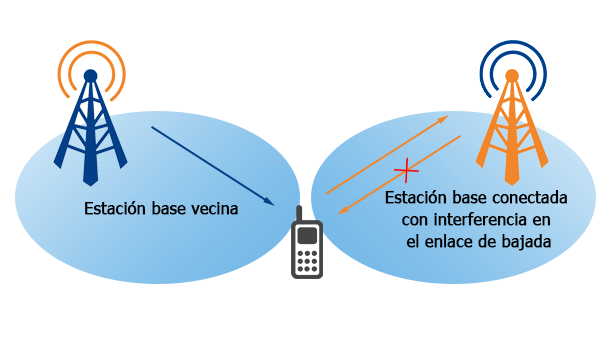
\includegraphics[width=0.75\linewidth]{imagenes/icic.png}
	\caption{Escenario simple en el que se utiliza una técnica de \acs{icic} para evitar interferencia en el enlace de bajada.}
	\label{fig:icic}
\end{figure}

Como se ha comentado anteriormente y como también se mostraba en el cuadro \ref{tab:5gfeatures}, los retos que se plantean para el desarrollo de 5G no son triviales. Con la finalidad de promover una investigación lo suficientemente eficaz como para abarcar todos los problemas que aparecen sobre la mesa, desde la Administración Pública se han consolidado programas impulsores como el Horizonte 2020 de la Unión Europea, el cual ofrece financiación para proyectos de cualquier naturaleza, incluidos los proyectos de \ac{tic}. Específicamente, el interés en el área \acs{tic} del Horizonte 2020 es conseguir los suficientes avances de consolidación de 5G y de infraestructuras \acs{tic} modernas, sobre todo si explotan el paradigma y/o hacen uso de entornos de IoT, Smart Cities o Big Data, a la vez que se hace hincapié en la ciberseguridad.

Gracias a dicha financiación, pueden ver la luz proyectos como \textit{QuaDRiGa} \cite{quadriga}, un simulador de canal escrito para la plataforma \textit{Matlab} que permite obtener datos realistas de comunicaciones basadas en entornos 5G y \acs{hetnet}. Dicho software será utilizado en este Trabajo de Fin de Grado y, por ello, se dedicará el Capítulo \ref{cap.quadriga} a analizarlo y describirlo con el suficiente detenimiento.

\section{Motivación}

Tal y como se habrá podido deducir de la sección anterior, un reto que suponen las redes heterogéneas es la complejidad de su planificación. El despliegue de numerosas \textit{small cells} junto a las celdas convencionales o nuevas \textit{large cells} agregan un esfuerzo adicional a la hora del diseño de las redes. Es obvia la necesidad de conocer el rendimiento a priori de las redes antes de su desdoble debido a su gran coste y a la suma importancia de ofrecer un servicio óptimo, sin sobredimensionar a la misma vez que se abastece a los usuarios sin sobrecargas.
Además, para un correcto desarrollo de los estándares venideros, como \acs{5g}, es preciso tener en mente los requisitos demandados por el futuro uso de los mismos. No es posible realizar un diseño de un estándar con tanto potencial como 5G sin una reproducción de resultados fiable.

Debido a tal problemática, en etapas de diseño, desarrollo, planificación y despliegue de redes y nuevas tecnologías inalámbricas, los simuladores toman un papel muy importante, puesto que permiten anticiparse a resultados con la finalidad de evitar futuros inconvenientes que un mal diseño pueda provocar, y su consecuente repercusión económica. Del mismo modo, los simuladores también permiten conocer los propios límites de una tecnología y su rendimiento. Algo que aunque solamente tenga un uso inmediato en los campos de investigación, a largo plazo permite evolucionar gracias a revisiones de dichas tecnologías y mejoras en siguientes versiones.

Es por ello que la finalidad del presente Trabajo de Fin de Grado es la elaboración de un simulador de comunicaciones móviles de entornos heterogéneos, con enfoque en \acs{5g}, llamado \textit{5Gneralife} -\textit{5G geNERAtor of LInk level simulations For Educational purposes}-.

\section{Objetivos}

El principal objetivo de este proyecto es utilizar como base el generador de canal de radio \textit{QuaDRiGa} utilizando la plataforma de programación y desarrollo \textit{Matlab} para el desarrollo de un simulador funcional de \acs{5g} que, como elementos fundamentales, incluya terminales móviles y \ac{bs} de tipo micro-celda y macro-celda, a la vez que permita obtener resultados básicos -potencia recibida, interferencias, capacidad de canal...- para distintos criterios de emparejamiento entre estaciones base, y terminales.

Para ello, en primer lugar el alumno debe familiarizarse con el entorno de \textit{QuaDriGa}, teniendo en cuenta que es un simulador de nivel de enlace que está capacitado para su uso a nivel de sistema, así como con el paradigma de comunicaciones móviles, indagando en 5G y en redes heterogéneas especialmente para conocer sus conceptos, metodologías y técnicas.

Seguidamente, es necesario hacer una planificación de las características que el simulador reunirá, descartando las que resulten inviables o aquellas que \textit{QuaDRiGa} no haga posible e implementarlas, modificando el código fuente de \textit{QuaDRiGa} si fuera necesario, y desarrollando sus propios \textit{scripts} y funciones.

El objetivo fundamental de estas etapas es el de extender el simulador de capa física \textit{QuaDRiGa} para obtener un simulador de nivel de enlace más completo con nuevas funcionalidades, incluyendo algunas características propias de simuladores de nivel de sistema, así como también una mayor flexibilidad para evaluar escenarios multi-celda y multi-frecuencia.

Por último, en base al trabajo realizado y al software implementado, se realizarán las oportunas pruebas comprobando el rendimiento de distintos escenarios y ajustes de comunicaciones, así como una especificación de orientaciones de uso para que las simulaciones resulten realistas.

\section{Organización de la memoria}

A modo de antesala del contenido del proyecto, a continuación se detalla un listado de capítulos y un resumen de sus contenidos, con la finalidad de aclarar qué se puede esperar en el proyecto y su organización.

\paragraph{Capítulo 1: Introducción} \mbox{} \\
	Este capítulo está dedicado a introducir la motivación del proyecto, su importancia y sus objetivos, así como realizar una primera toma de contacto con las herramientas que se utilizarán. También se realiza una descripción de la organización de la memoria.

\paragraph{Capítulo 2: Estado del arte} \mbox{} \\
	En él se describen las soluciones que existen en la actualidad en cuanto a simuladores 5G se refiere. Se realiza una breve evaluación de los principales simuladores 5G, independientemente de su clasificación.

\paragraph{Capítulo 3: Planificación y requisitos} \mbox{} \\
	Se establecen unos requisitos que se consideran imprescindibles para que, una vez dada la finalización del proyecto, este resulte satisfactorio. Además, se expone la planificación que se llevó a cabo para la realización del proyecto así como una estimación del coste que conllevaría.

\paragraph{Capítulo 4: Acerca de \textit{QuaDRiGa}} \mbox{} \\
	En este capitulo se lleva a cabo una descripción detallada de \textit{QuaDRiGa}, exponiendo sus funcionalidades, limitaciones, su paradigma de programación y su estructura. Finalmente, se realiza una pequeña prueba de dicho software.

\paragraph{Capítulo 5: Diseño e implementación} \mbox{} \\
    Este capítulo contiene una explicación detallada de toda la funcionalidad del código del proyecto, su diseño y estructura, una descripción de sus características y funcionalidades y, por último, una guía de uso.

\paragraph{Capítulo 6: Pruebas} \mbox{} \\
    Se realiza una serie de pruebas al simulador para comprobar su capacidad y evaluar los resultados obtenidos así como el consumo de recursos. También se extraen observaciones y características de los entornos simulados.

\paragraph{Capítulo 7: Conclusiones} \mbox{} \\
    Conclusiones, defectos y puntos fuertes \textit{5Gneralife}. Alcance del proyecto. Se detallan posibles mejoras y futuros pasos para el proyecto, así como sus perspectivas de futuro.

%\section{Alcance del trabajo}